\begin{block}{Synchronisation des micro-structures}
    Dans le cas d'une exécution partagée d'un scénario, il convient de définir la sémantique d'exécution des points de synchronisation, des conditions, et des vitesses de contraintes, en mode réparti. 
   
    C'est fait via deux caractéristiques:~\\
    La \textbf{synchronisation}~:
	\begin{itemize}
		\item \textbf{Mode synchrone}~: on respecte la sémantique d'exécution des partitions interactives au prix d'une latence de synchronisation.
		\item \textbf{Mode asynchrone}~: on ne respecte pas la sémantique avant-après. La fin de l'exécution d'un objet peut survenir quelques millisecondes après le début de l'exécution de l'objet suivant.
	\end{itemize}

Le \textbf{délai de propagation}~:
\begin{itemize}
    \item \textbf{Propagation instantanée}~: dès qu'une information est disponible dans le système, les clients qui en dépendent en sont informés et peuvent y réagir immédiatement. 
    \item \textbf{Propagation compensée}~: quand une information est disponible dans le système, on estime la date minimale à partir de laquelle tous les clients peuvent être informés en fonction de la latence entre machines. 
    Elles reçoivent toutes un ordre qu'elles sont sensées exécuter à cette date. 
    C'est utile si on désire par exemple une bonne synchronisation entre vidéos.
\end{itemize}

Via des annotations, le compositeur peut définir le type de répartition qu'il souhaite sur chaque objet.

\begin{figure}
	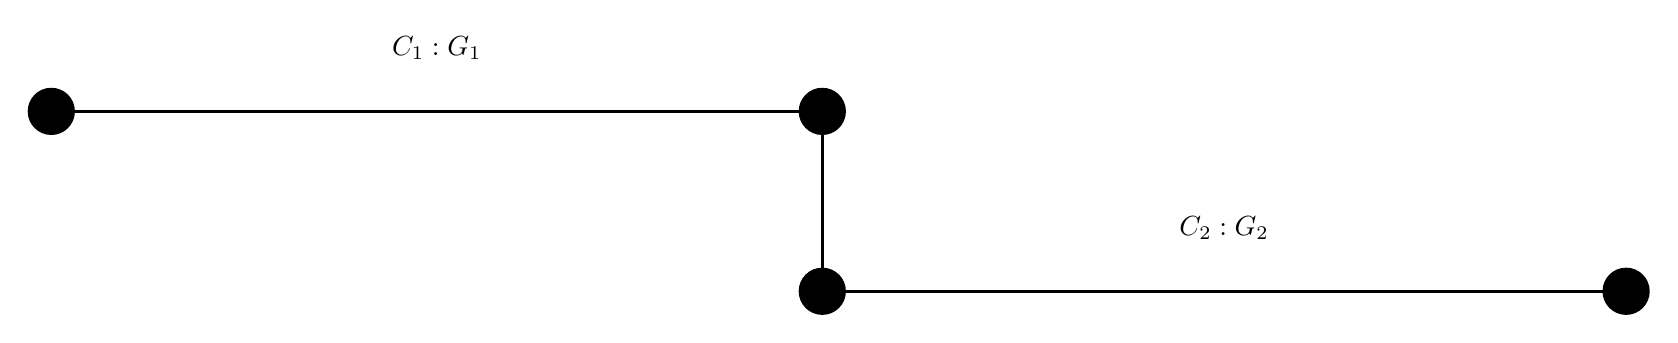
\begin{tikzpicture}[scale=4]
	\fill (0, 9.98122) circle (0.075) ; % State.0 
\fill (2.44792, 9.98122) circle (0.075) ; % State.1 
\fill (2.44792, 9.41005) circle (0.075) ; % State.2 
\fill (5, 9.41005) circle (0.075) ; % State.3 
\draw[line width=1pt] (0, 9.98122)  -- (0, 9.98122) ; % TimeNode.0 
\draw[line width=1pt] (2.44792, 9.98122)  -- (2.44792, 9.41005) ; % numb47vine94 
\draw[line width=1pt] (5, 9.41005)  -- (5, 9.41005) ; % faze44greg1 
\draw[line width=1pt] (0, 9.98122)  -- (2.44792, 9.98122) ; % dido10rend91 
\draw (1.22396, 10.1812) node {$C_1: G_1$}; % dido10rend91 
\draw[line width=1pt] (2.44792, 9.41005)  -- (5, 9.41005) ; % taut8hews94 
\draw (3.72396, 9.61005) node {$C_2: G_2$}; % taut8hews94 

	\end{tikzpicture}
	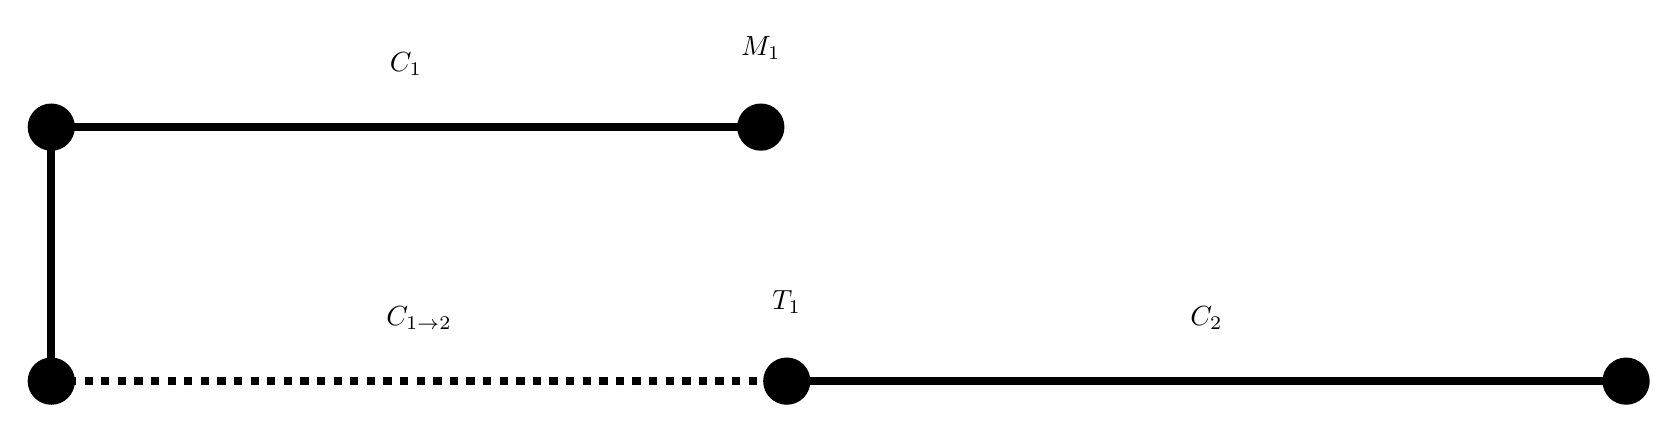
\begin{tikzpicture}[scale=4]
	\fill (0, 12.3782) circle (0.075) ; % State.0 
\fill (2.25275, 12.3782) circle (0.075) ; % State.1 
\fill (0, 11.5717) circle (0.075) ; % State.2 
\fill (2.33516, 11.5717) circle (0.075) ; % State.3 
\fill (5, 11.5717) circle (0.075) ; % State.4 
\draw[line width=3pt] (0, 12.3782)  -- (0, 11.5717) ; % TimeNode.0 
\draw[line width=3pt] (2.25275, 12.3782)  -- (2.25275, 12.3782) ; % said66toil5 
\draw (2.25275, 12.6282) node {$M_1$}; % said66toil5 
\draw[line width=3pt] (2.33516, 11.5717)  -- (2.33516, 11.5717) ; % dear17tick57 
\draw (2.33516, 11.8217) node {$T_1$}; % dear17tick57 
\draw[line width=3pt] (5, 11.5717)  -- (5, 11.5717) ; % pane76toll8 
\draw[line width=3pt] (0, 12.3782)  -- (2.25275, 12.3782) ; % mask27tara32 
\draw (1.12637, 12.5782) node {$C_1$}; % mask27tara32 
\draw[dashed,line width=3pt] (0, 11.5717)  -- (2.33516, 11.5717) ; % acid4ball90 
\draw (1.16758, 11.7717) node {$C_{1\rightarrow2}$}; % acid4ball90 
\draw[line width=3pt] (2.33516, 11.5717)  -- (5, 11.5717) ; % ride82vine29 
\draw (3.66758, 11.7717) node {$C_2$}; % ride82vine29 

	\end{tikzpicture}
	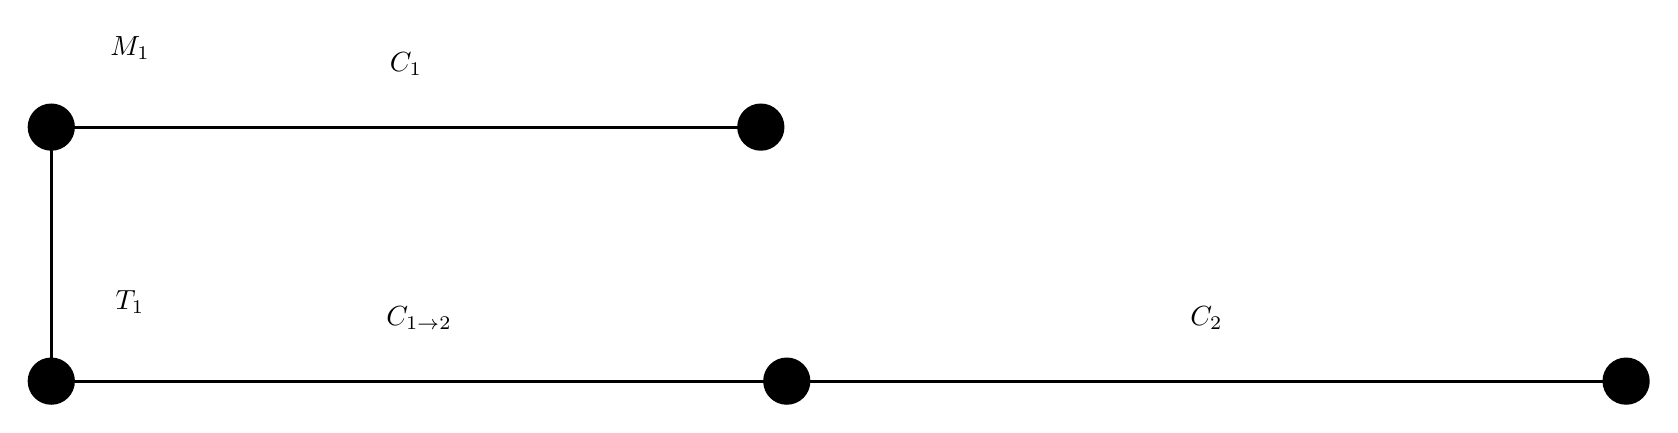
\begin{tikzpicture}[scale=4]
	\fill (0, 12.3782) circle (0.075) ; % State.0 
\fill (2.25275, 12.3782) circle (0.075) ; % State.1 
\fill (0, 11.5717) circle (0.075) ; % State.2 
\fill (2.33516, 11.5717) circle (0.075) ; % State.3 
\fill (5, 11.5717) circle (0.075) ; % State.4 
\draw (0.25, 12.6282) node {$M_1$};
\draw[line width=1pt] (0, 12.3782)  -- (0, 11.5717) ; % TimeNode.0 
\draw (0.25, 11.8217) node {$T_1$};
\draw[line width=1pt] (2.25275, 12.3782)  -- (2.25275, 12.3782) ; % said66toil5 
\draw[line width=1pt] (2.33516, 11.5717)  -- (2.33516, 11.5717) ; % dear17tick57 
\draw (2.33516, 11.8217) node {}; % dear17tick57 
\draw[line width=1pt] (5, 11.5717)  -- (5, 11.5717) ; % pane76toll8 
\draw[line width=1pt] (0, 12.3782)  -- (2.25275, 12.3782) ; % mask27tara32 
\draw (1.12637, 12.5782) node {$C_1$}; % mask27tara32 
\draw[line width=1pt] (0, 11.5717)  -- (2.33516, 11.5717) ; % acid4ball90 
\draw (1.16758, 11.7717) node {$C_{1\rightarrow2}$}; % acid4ball90 
\draw[line width=1pt] (2.33516, 11.5717)  -- (5, 11.5717) ; % ride82vine29 
\draw (3.66758, 11.7717) node {$C_2$}; % ride82vine29 

	\end{tikzpicture}
	\caption{De haut en bas : la partition que le compositeur exprime, sa version lorsque répartie en mode asynchrone pré-calculé et sa version lorsque répartie en mode synchrone compensé.}
\end{figure}
\end{block}